\chapter{Установка редактора исходного кода Code::Blocks}
Для написания собственных программ на языке программирования C\texttt{++} необходимо установить любую из возможных сред разработки. Например, свободную кроссплатформенную среду разработки --- \textbf{Code::Blocks}.
\begin{itemize}
    \item Скачиваем дистрибутив с сайта {\color{Blue}\href{https://www.codeblocks.org/downloads/binaries/#imagesoswindows48pnglogo-microsoft-windows}{codeblocks.org}}.
    \item После установки на рабочем столе появляется иконка с одноименным названием, или же в меню \textbf{Пуск$\rightarrow$Все программы}.
    \item В открывшемся окне выбираем \textbf{Create a new project}
    \begin{figure}[H]
        \centering
        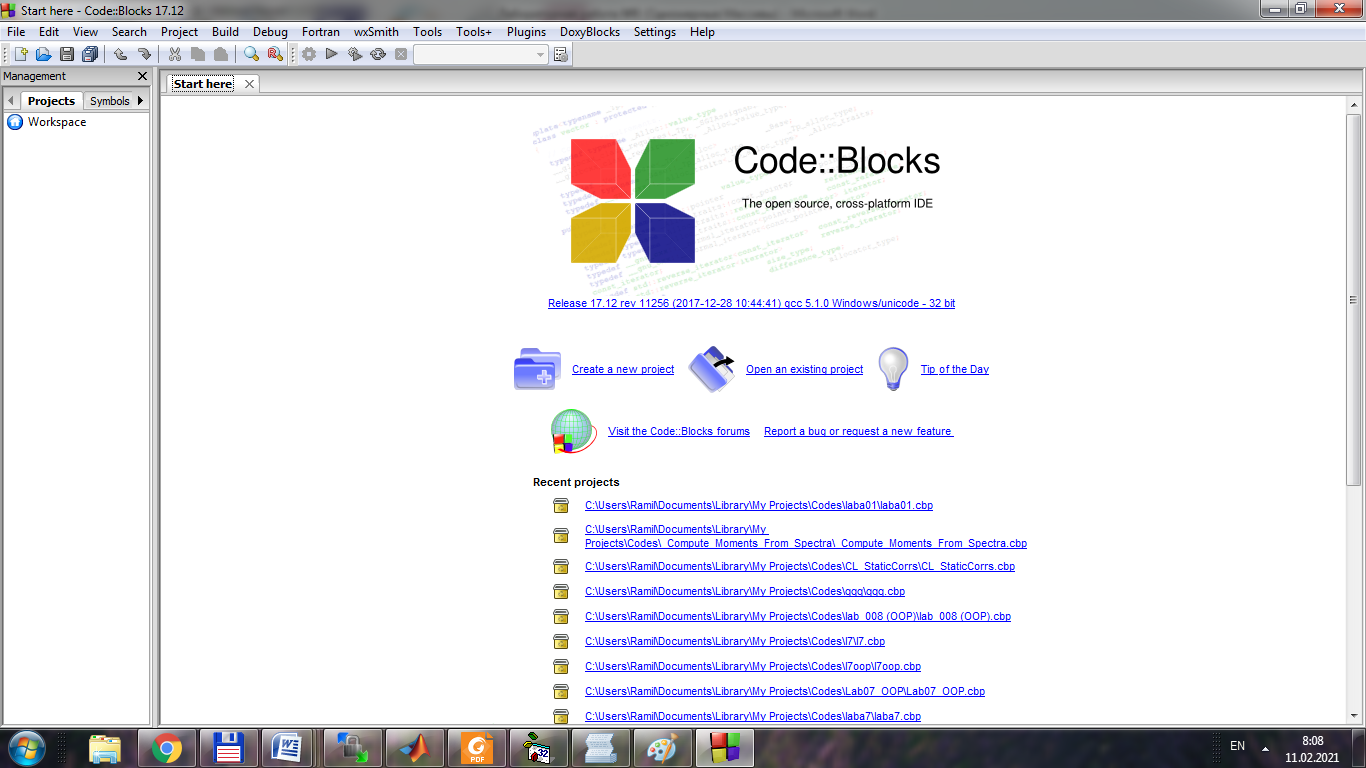
\includegraphics[width=.9\linewidth]{figures/CodeBlocks-1.png}
        \caption{Запуск программы Code::Blocks}
        \label{CodeBlocks-1}
    \end{figure}
    \item Выбираем иконку \textbf{Console Application}
    \begin{figure}[H]
        \centering
        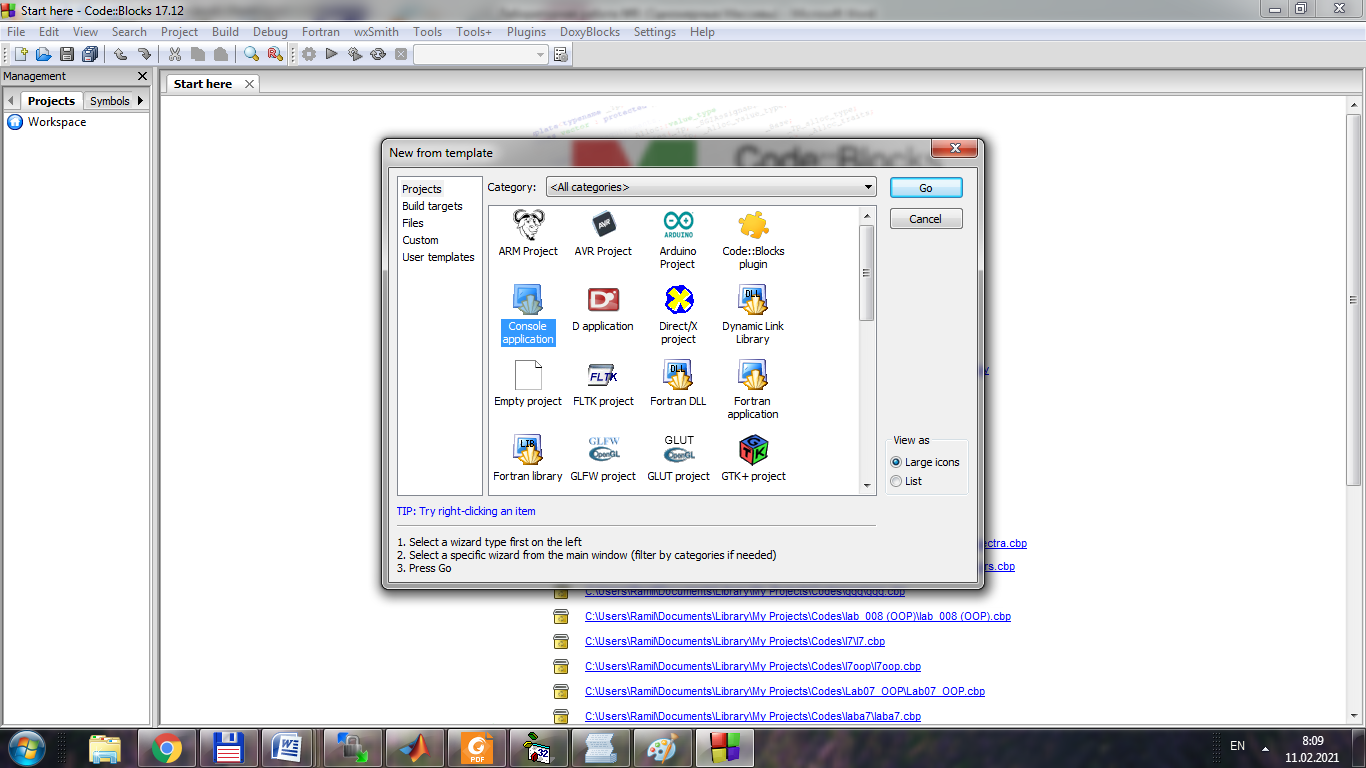
\includegraphics[width=.9\linewidth]{figures/CodeBlocks-2.png}
        \caption{Окно выбора иконки Console Application}
        \label{CodeBlocks-2}
    \end{figure}
    \item Выбираем \textbf{C\texttt{++}}
    \begin{figure}[H]
        \centering
        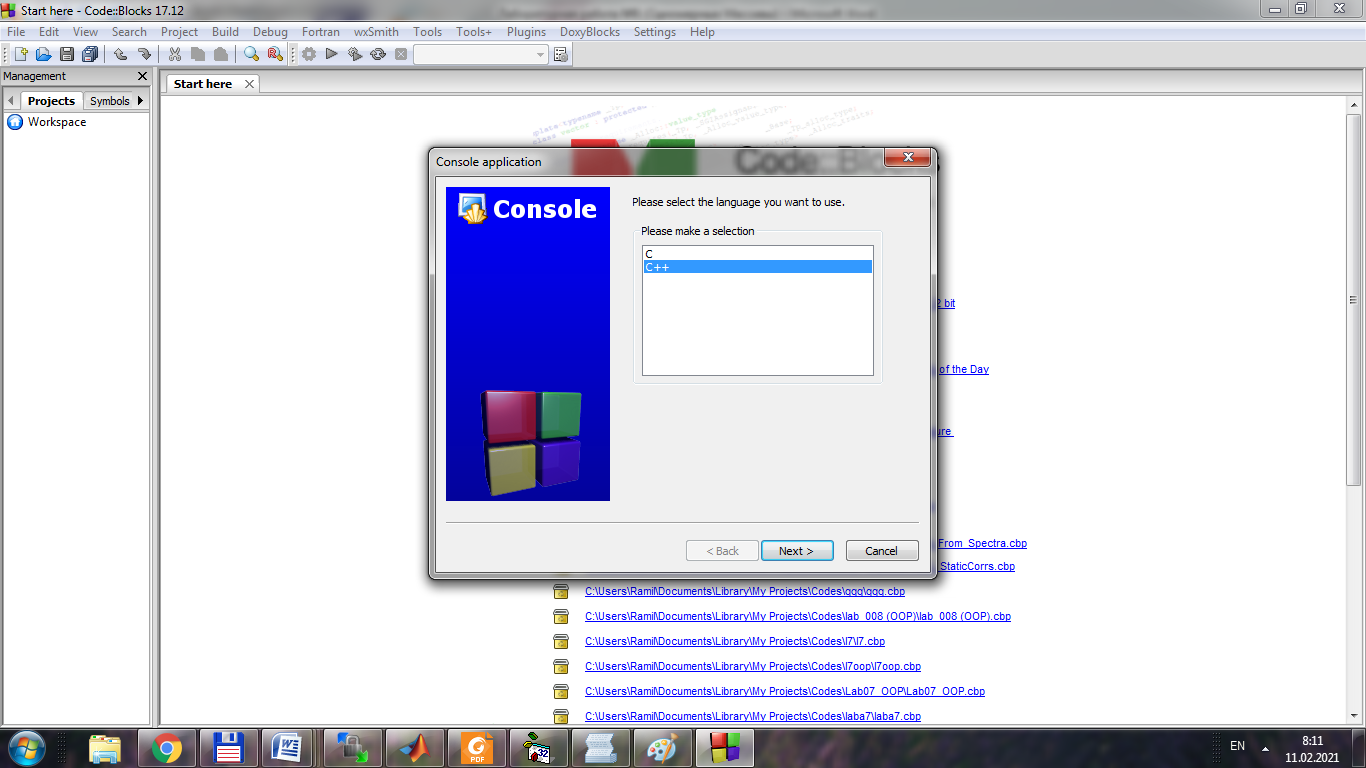
\includegraphics[width=.9\linewidth]{figures/CodeBlocks-3.png}
        \caption{Выбор языка C\texttt{++}}
        \label{CodeBlocks-3}
    \end{figure}
    \item Пишем имя проекта, например, \textbf{\_\_lab01}
    \begin{figure}[H]
        \centering
        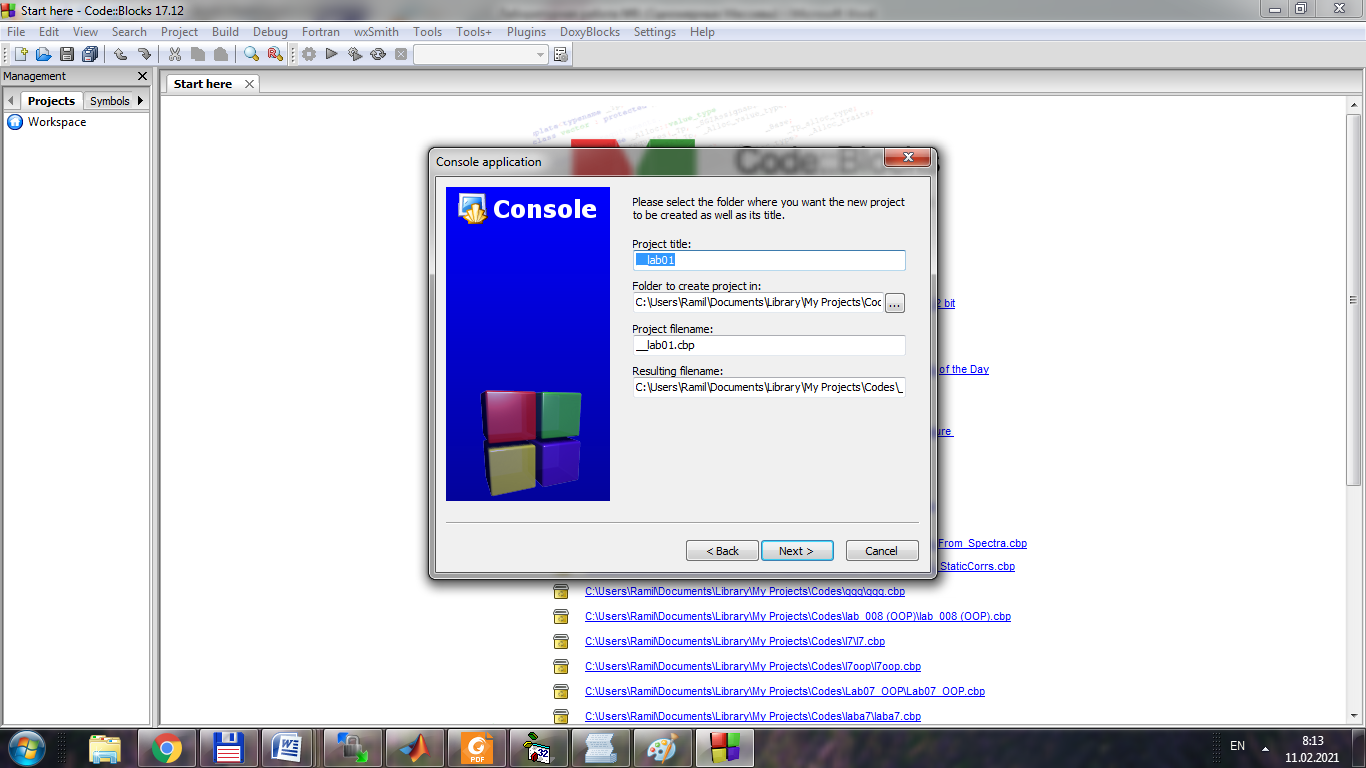
\includegraphics[width=.9\linewidth]{figures/CodeBlocks-4.png}
        \caption{Ввод имени проекта}
        \label{CodeBlocks-4}
    \end{figure}
    \item Далее, соглашаемся на все предложенные варианты, и кликаем на вкладку \textbf{Sources}$\rightarrow$ \textbf{main.cpp}. В результате, получаем следующее окно и шаблон программы \textbf{Hello, world!}
    \begin{figure}[H]
        \centering
        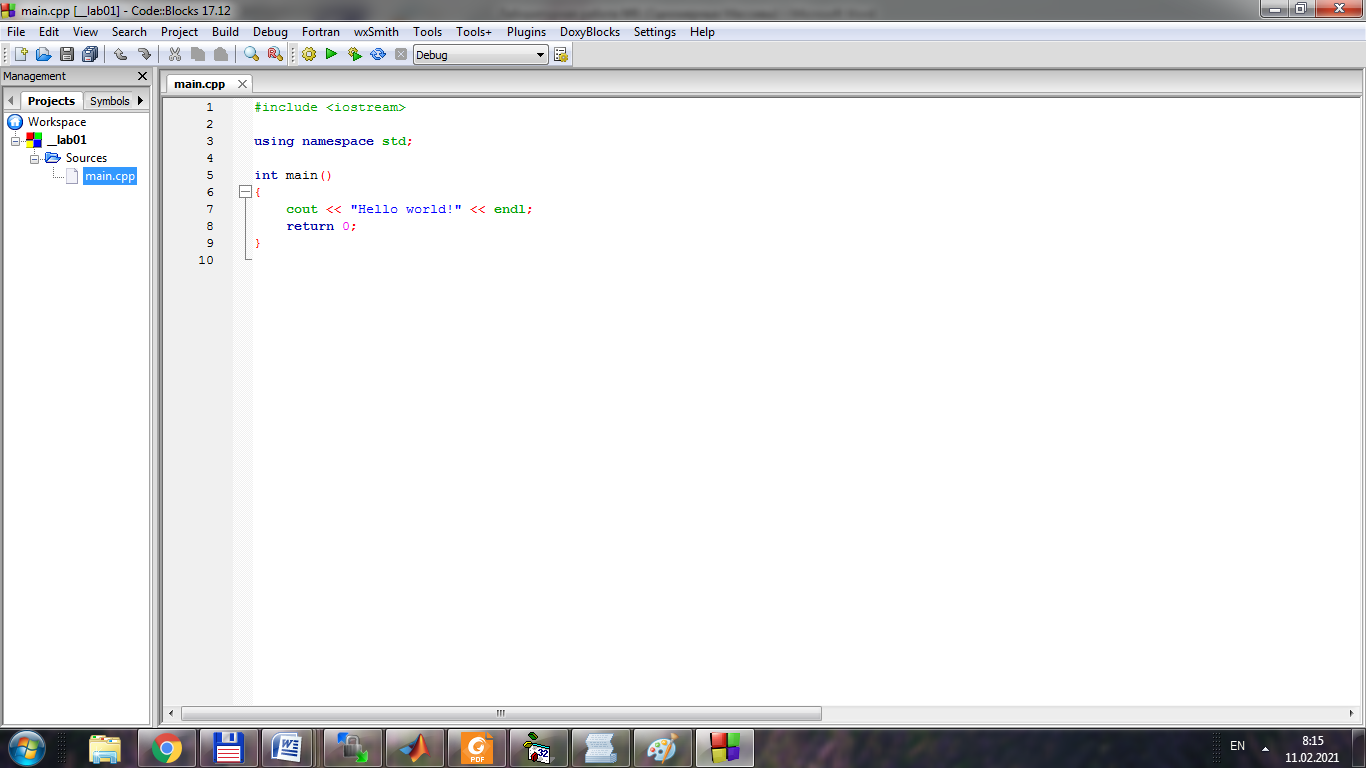
\includegraphics[width=.9\linewidth]{figures/CodeBlocks-5.png}
        \caption{Программа <<Hello, world!>> в окне редактора исходного кода}
        \label{CodeBlocks-5}
    \end{figure}
    \item Для компиляции и запуска программы нажимаем на клавишу \textbf{F9} (\textbf{Build and run}).
\end{itemize}